\providecommand{\setflag}{\newif \ifwhole \wholefalse}
\setflag
\ifwhole\else

% Typography and geometry ----------------------------------------------------
\documentclass[letterpaper]{scrbook}
\usepackage[inner=3cm,top=2.5cm,outer=3.5cm]{geometry}

\renewcommand\familydefault{bch}
\usepackage[utf8]{inputenc}
\usepackage{microtype}
\usepackage[small]{caption}
\usepackage[small]{titlesec}
\raggedbottom

% Graphics -------------------------------------------------------------------
\usepackage[pdftex]{graphicx}
\graphicspath{{_include/}}
\DeclareGraphicsExtensions{.png,.pdf}

% Code formatting ------------------------------------------------------------
\usepackage{fancyvrb}
\usepackage{courier}
\usepackage{listings}
\usepackage{color}
\usepackage{alltt}


\definecolor{comment}{rgb}{0.60, 0.60, 0.53}
\definecolor{background}{rgb}{0.97, 0.97, 1.00}
\definecolor{string}{rgb}{0.863, 0.066, 0.266}
\definecolor{number}{rgb}{0.0, 0.6, 0.6}
\definecolor{variable}{rgb}{0.00, 0.52, 0.70}
\lstset{
  basicstyle=\ttfamily,
  keywordstyle=\bfseries, 
  identifierstyle=,  
  commentstyle=\color{comment} \emph,
  stringstyle=\color{string},
  showstringspaces=false,
  columns = fullflexible,
  backgroundcolor=\color{background},
  mathescape = true,
  escapeinside=&&,
  fancyvrb
}
\newcommand{\code}[1]{\lstinline!#1!}
\newcommand{\f}[1]{\lstinline!#1()!}



% Links ----------------------------------------------------------------------

\usepackage{hyperref}
\definecolor{slateblue}{rgb}{0.07,0.07,0.488}
\hypersetup{colorlinks=true,linkcolor=slateblue,anchorcolor=slateblue,citecolor=slateblue,filecolor=slateblue,urlcolor=slateblue,bookmarksnumbered=true,pdfview=FitB}
\usepackage{url}

% Tables ---------------------------------------------------------------------
\usepackage{longtable}
\usepackage{booktabs}

% Miscellaneous --------------------------------------------------------------
\usepackage{pdfsync}
\usepackage{appendix}

\usepackage[round,sort&compress,sectionbib]{natbib}
\bibliographystyle{plainnat}


\title{ggplot2}
\author{Hadley Wickham}

\begin{document}
\fi

% SET_DEFAULTS
%   GG-WIDTH: 4  GG-HEIGHT: 4
%   TEX-WIDTH: 0.5\linewidth COL: 2
%   INLINE: FALSE
%   CACHE: TRUE
% 

% END

\chapter{Positioning}
\label{cha:position}

\section{Introduction}

This chapter discusses position, particularly how facets are laid out on a page, and how coordinate systems within a panel work.  There are four components that control position.  You have already learned about two of them that work within a facet:

\begin{itemize}
  \item {\bf Position adjustments} adjust the position of overlapping objects within a layer, and were described in Section~\ref{sec:position}.  These are most useful for bar and other interval geoms, but can be useful in other situations.

  \item {\bf Position scales}, previously described in Section~\ref{sub:scale-position}, control how the values in the data are mapped to positions on the plot.  Common transformations are linear and log, but any other invertible function can also be used.
\end{itemize}

\noindent This chapter will describe the other two components and show you how all four components can be used together:

\begin{itemize}
  \item {\bf Faceting}, described in Section~\ref{sec:faceting}, is a mechanism for automatically laying out multiple plots on a page.  It splits the data into subsets, and then plots each subset into a different panel on the page.  Such plots are often called small multiples.  

  \item {\bf Coordinate systems}, described in Section~\ref{sec:coord}, control how the two independent position scales are combined to create a 2d coordinate system.  The most common coordinate system is Cartesian, but other coordinate systems can be useful in special circumstances.

\end{itemize}

\section{Faceting}
\label{sec:faceting}

You first encountered faceting in the introduction to \f{qplot}, Section~\ref{sec:qplot-faceting}, and you may already have been using it in your plots.  Faceting generates small multiples each showing a different subset of the data.  Small multiples are a powerful tool for exploratory data analysis: you can rapidly compare patterns in different parts of the data and see whether they are the same or different.  This section will discusses how you can fine tune facets, particularly in the way in which they interact with position scales. 

There are two types of faceting provided by \ggplot: \code{facet_grid} and \code{facet_wrap}.  Facet grid produces a 2d grid of panels defined by variables which form the rows and columns, and while facet wrap produces 1d ribbon of panels that is wrapped into 2d.  The grid layout is similar to the layout of \code{coplot} in base graphics, and the wrapped layout is similar to the layout of panels in \code{lattice}.  These differences are illustrated in Figure~\ref{fig:facets-sketch}.

\begin{figure}[htbp]
  \centering
    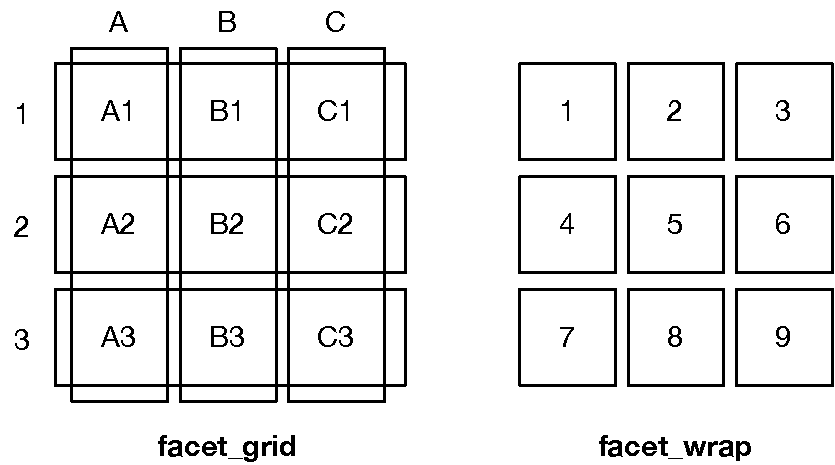
\includegraphics[width=0.5\linewidth]{position-facets}
  \caption{A sketch illustrating the difference between the two faceting systems.   \f{facet_grid} (left) is fundamentally two-d, being made up of two independent components.  \f{facet_wrap} (right) is one-d, but wrapped into two-d to save space.}
  \label{fig:facet-sketch}
\end{figure}

There are two basic arguments to the faceting systems: the variables to facet by, and whether position scales should global or local to the facet.  The way these options are specified is a little different for the two systems, so they are described separately below.

% Faceting can be thought of a special type of coordinate system, one that is hierarchical.  At the top level we have a coordinate system created by the categorical variables that we are faceting by, and then within each of these regions another coordinate system generated by the x and y position of each graphic.

You can access either faceting system from \f{qplot}. A 2d faceting specification (e.g.\ \code{x ~ y}) will use \code{facet_grid}, while a 1d specification (e.g.\ \verb|~ x|) will use \code{facet_wrap}.

Facetted plots have the capability to fill up a lot of space, so for this chapter we will use a subset of the mpg dataset that has a manageable number of levels: three cylinders (4, 6, 8) and two types of drive train (4 and f).  This removes 29 vehicles from the original dataset.

% INTERWEAVE
%
% mpg2 <- subset(mpg, cyl != 5 & drv %in% c("4", "f"))
\input{_include/e801ae8d479ec9884e584f1f0e81f4ce.tex}
% END

\subsection{Facet grid}

The grid faceter lays out plots in a 2d grid.  When specifying a faceting formula, you specify which variables should appear in the columns and which should appear in the rows, as follows:  

\begin{itemize}
  \item \code{. ~ .}   The default. Neither rows nor columns are faceted, so you get a single panel.

  % INTERWEAVE
  % 
  % qplot(cty, hwy, data = mpg2) + facet_grid(. ~ .)
  \input{_include/74200320eea8c281c5289e5bda7e7420.tex}  
  % END

  \item \code{. ~ a} A single row with multiple columns.  This is normally the most useful direction because computer screens are usually wider than they are long.  This direction of faceting facilitates comparisons of y position, because the vertical scales are aligned.

  % INTERWEAVE
  %   GG-WIDTH: 9 GG-HEIGHT: 3  TEX-WIDTH: \linewidth
  % 
  % qplot(cty, hwy, data = mpg2) + facet_grid(. ~ cyl)
  \input{_include/6d6285ec25eb06d8061e1256c609a226.tex}  
  % END
  
  \item \code{b ~ .} A single column with multiple rows.  This direction facilitates comparison of x position, because the horizontal scales are aligned, and so is particularly useful for comparing distributions.  Figure~\ref{fig:facet-hist} on page \pageref{fig:facet-hist} is a good example of this use.

  % INTERWEAVE
  % 
  % qplot(cty, data = mpg2, geom="histogram", binwidth = 2) +
  %   facet_grid(cyl ~ .)
  \input{_include/1644f7602c0c53dfaf6734b1cce6a509.tex}  
  % END

  \item \code{a ~ b}: Multiple rows and columns.  You'll usually want to put the variable with the greatest number of levels in the columns, to take advantage of the aspect ratio of your screen.

  % INTERWEAVE
  %   GG-WIDTH: 8 GG-HEIGHT: 3  TEX-WIDTH: \linewidth
  % 
  % qplot(cty, hwy, data = mpg2) + facet_grid(drv ~ cyl)
  \input{_include/182e936da01c02f0a7b6645821e487a2.tex}  
  % END

  \item \code{. ~ a + b} or \code{a + b ~ .}  Multiple variables in the rows or columns (or both). This is unlikely to be useful unless the number of factor levels is small, you have a very wide screen, or you want to produce a long, skinny poster.

  % INTERWEAVE
  %   GG-WIDTH: 12 GG-HEIGHT: 3  TEX-WIDTH: \linewidth
  % 
  % qplot(cty, hwy, data = mpg2) + facet_grid(. ~ cyl + drv)
  \input{_include/39c6a0bd3169a5d55cdc45b752347b3f.tex}  
  % END

\end{itemize}

Variables appearing together on the rows or columns are nested in the sense that only combinations that appear in the data will appear in the plot.  Variables that are specified on rows and columns will be crossed: all combinations will be shown, including those that didn't appear in the original data set: this may result in empty panels.

\subsubsection{Margins}\label{sub:margins}

Faceting a plot is like creating a contingency table.  In contingency tables it is often useful to display marginal totals (totals over a row or column) as well as the individual cells.  It is also useful to be able to do this with graphics, and you can do so with the {\tt margins} argument.  This allows you to compare the conditional patterns with the marginal patterns.

You can either specify that all margins should be displayed, using {\tt margins = TRUE}, or by listing the names of the variables that you want margins for, {\tt margins = c("sex", "age")}.  You can also use \verb|"grand_row"| or \verb|"grand_col"| to produce grand row and grand column margins respectively.  

Figure~\ref{fig:margins} shows what margins look like.  The first plot shows what the data looks like without margins, and the second shows all margins.  The margin column shows all drive trains, the margin row shows all cylinders, and the bottom-right plot (the grand total) shows the full data set.  For this data we can see that as the number of cylinders increases, engine displacement increases and fuel economy decreases, and compared to front wheel drive vehicles, as a group four wheel drive vehicles have about the same displacement, but are less fuel efficient.  The figure was produced with the following code:

% FIGLISTING
%   FILETYPE: PNG
%   LABEL: margins
%   CAPTION: Graphical margins work like margins of a contingency table to
%   give unconditioned views of the data.  A plot facetted by number of 
%   cylinders and drive train (left) is supplemented with margins (right).
% 
% p <- qplot(displ, hwy, data = mpg2) +
%   geom_smooth(method = "lm", se = F)
% p + facet_grid(cyl ~ drv) 
% p + facet_grid(cyl ~ drv, margins = T)
\input{_include/bec2e450278a8841cafc9f41fca2d70c.tex}
% END

Groups in the margins are controlled in the same way as groups in all other panels, defaulting to the interaction of all categorical variables present in the layer.  (See Section~\ref{sub:grouping} for a reminder.)  The following example shows what happens when we add a coloured smooth for each drive train. 

% INTERWEAVE
%   FILETYPE: PNG
% 
% qplot(displ, hwy, data = mpg2) + 
%   geom_smooth(aes(colour = drv), method = "lm", se = F) + 
%   facet_grid(cyl ~ drv, margins = T) 
\input{_include/9754c4ca66f9d8638e141bdcec25d746.tex}
% END

Plots with many facets and margins may be more appropriate for printing than on screen display, as the higher resolution of print (600 dpi vs 72 dpi) allows you to compare many more subsets.

\subsection{Facet wrap}
\label{sub:facet_wrap}

An alternative to the grid is a wrapped ribbon of plots.  Instead of having a 2d grid generated by the combination of two (or more) variables, \code{facet_wrap} makes a long ribbon of panels (generated by any number of variables) and wraps it into 2d.  This is useful if you have a single variable that with many levels and want to arrange the plots in a more space efficient manner.  This is what trellising in lattice does.

Figure~\ref{fig:movies-wrap} shows the distribution of average movie ratings by decade. The main difference over time seems to be the increasing spread of ratings. This is probably an artefact of the number of votes: newer movies get more votes and so the average ratings are likely to be less extreme. The disadvantage of this style of faceting is that it is harder to compare some subsets that should be close together, as in this example where the plots for the 50's and 60's are particularly far apart because of the way the ribbon has been wrapped around. The figure was produced with the following code:

% FIGLISTING
%   COL: 1 GG-WIDTH: 10 TEX-WIDTH: \linewidth
%   LABEL: movies-wrap
%   CAPTION: Movie rating distribution by decade.
% 
% movies$decade <- round_any(movies$year, 10, floor)
% qplot(rating, ..density.., data=subset(movies, decade > 1890),
%   geom="histogram", binwidth = 0.5) + facet_wrap(~ decade, ncol = 6)
\input{_include/7ff6e48f78b0d4bb164bee4e946c5afa.tex}
% END

The specification of faceting variables is of the form \code{ \~ a + b + c}. By default, \code{facet_wrap} will try and layout the panels as close to a square as possible, with a slight bias towards wider rather than taller rectangles. You can override the default by setting \code{ncol}, \code{nrow} or both. See the documentation for more examples.

\subsection{Controlling scales}
\label{sub:controlling_scales}

For both types of faceting you can control whether the position scales are the same in all panels (fixed) or allowed to vary between panels (free).  This is controlled by the \code{scales} parameter:

\begin{itemize}
  \item \code{scales = "fixed"}: x and y scales are fixed across all panels
  \item \code{scales = "free"}: x and y scales vary across panels.
  \item \code{scales = "free_x"}: the x scale is free, and the y scale is fixed.
  \item \code{scales = "free_y"}: the y scale is free, and the x scale is fixed.
\end{itemize}

\noindent Figure~\ref{fig:fixed-vs-free} illustrates the difference between the two extremes of fixed and free.

% FIGLSTING
%   LABEL: fixed-vs-free
%   CAPTION: Fixed scales (left) have the same scale for each facet, while 
%   free scales (right) have a different scale for each facet. 
% 
% p <- qplot(cty, hwy, data = mpg)
% p + facet_wrap(~ cyl)
% p + facet_wrap(~ cyl, scales = "free")

Fixed scales allow us to compare subsets on an equal basis, seeing where each fits into the overall pattern.  Free scales zoom in on the region that each subset occupies, allowing you to see more details. Free scales are particularly useful when we want to display multiple times series that were measured on different scales.  To do this, we first need to change from ``wide'' to ``long'' data, stacking the separate variables into a single column.  An example of this is shown in Figure~\ref{fig:time}, and the topic is discussed in more detail in Section~\ref{sec:melting}.  

% FIGLISTING
%   COL: 1 GG-WIDTH: 10 TEX-WIDTH: \linewidth
%   LABEL: time
%   CAPTION: Free scales are particularly useful when displaying multiple 
%   time series that are measured on different scales.
% 
% em <- melt(economics, id = "date")
% qplot(date, value, data = em, geom = "line", group = variable) + 
%   facet_grid(variable ~ ., scale = "free_y")
\input{_include/a070a3fc50dc948499e26d8409b3c36c.tex}
% END

There is an additional constraint on the scales of \code{facet_grid}: all panels in a column must have the same x scale, and all panels in a row must have the same y scale.  This is because each column shares an x axis, and each row shares a y axis.

For \code{facet_grid} there is an additional parameter called \code{space}, which takes values \code{"free"} or \code{"fixed"}.  When the space can vary freely, each column (or row) will have width (or height) proportional to the range of the scale for that column (or row).  This makes the scaling equal across the whole plot: 1 cm on each panel maps to the same range of data.  (This is somewhat analogous to the ``sliced'' axis limits of lattice).  For example, if panel a had range 2 and panel b had range 4, one-third of the space would be given to a, and two-thirds to b.  This is most useful for categorical scales, where we can assign space proportionally based on the number of levels in each facet, as illustrated by Figure~\ref{fig:discrete-free}.  The code to create this plot is shown below: note the use of \f{reorder} to arrange the models and manufacturers in order of city fuel usage.

% FIGLISTING
%   COL: 2 GG-HEIGHT: 8 TEX-WIDTH: 0.5\linewidth
%   LABEL: discrete-free
%   CAPTION: A dotplot showing the range of city gas mileage for each model
%   of car. (Left) Models ordered by average mpg, and (right) faceted by
%   manufacturer with \code{scales="free_y"} and \code{space = "free"}.  The 
%   {\tt strip.text.y} theme setting has been used to rotate the facet labels.
% 
% mpg3 <- within(mpg2, {
%   model <- reorder(model, cty)
%   manufacturer <- reorder(manufacturer, -cty)
% })
% models <- qplot(cty, model, data = mpg3)
%
% models
% models + facet_grid(manufacturer ~ ., scales = "free", space = "free") +  
%   opts(strip.text.y = theme_text())
\input{_include/e750be5098f5267b3682b8cced7b3758.tex}
% END

\subsection{Missing faceting variables}
\label{sub:missing_faceting_columns}

If you using faceting on a plot with multiple datasets, what happens when one of those datasets is missing the faceting variables? This situation commonly arises when you are adding contextual information that should be the same in all panels. For example, imagine you have spatial display of disease faceted by gender. What happens when you add a map layer that does not contain the gender variable?  Here \ggplot will do what you expect: it will display the map in every facet: missing faceting variables are treated like they have all values.

% % INTERWEAVE
% %   COL: 1 GG-WIDTH: 8 TEX-WIDTH: 0.8\linewidth
% % 
% % ctyhwy <- qplot(cty, hwy, data = mpg2) + facet_grid(. ~ cyl)
% % ctyhwy
% % 
% % # Extract best & worst
% % extreme_global <- subset(mpg2, rank(cty) < 5)
% % extreme <- subset(mpg2, cty < 12 | cty > 30)[c("cty", "hwy", "cyl")]
% % 
% % # Show extremes on all facets (remove cyl column)
% % ctyhwy + geom_point(data = extreme[, 1:2], colour = "red", size = 2)
% % # Show extremes for each facet (keep cyl column)
% % ctyhwy + geom_point(data = extreme, colour = "red", size = 2)
% \input{_include/05ca8013028096d11fa34a73dcafa7df.tex}
% % END

\subsection{Grouping vs. faceting}
\label{sub:group-vs-facet}

Faceting is an alternative to using aesthetics (like colour, shape or size) to differentiate groups. Both techniques have strengths and weaknesses, based around the relative positions of the subsets. 

With faceting, each group is quite far apart in its own panel, and there is no overlap between the groups.  This is good if the groups overlap a lot, but it does make small differences harder to see.  When using aesthetics to differentiate groups, the groups are close together and may overlap, but small differences are easier to see.  Figure~\ref{fig:group-vs-facet} illustrates these trade-offs.  With the scatterplots, it is possible to not realise the groups are overlapping when just colour is used to separate them, but with the regression lines they are too far apart to see that D, E and G are grouped together and J is further away.  The code to produce these figures is shown below.

% FIGLISTING
%   LABEL: group-vs-facet
%   CAPTION: The differences between faceting vs grouping, illustrated with
%   a log-log plot of carat vs price with four selected colours.
%   FILETYPE: png
% 
% xmajor <- c(0.3, 0.5, 1,3, 5)
% xminor <- as.vector(outer(1:10, 10^c(-1, 0)))
% ymajor <- c(500, 1000, 5000, 10000)
% yminor <- as.vector(outer(1:10, 10^c(2,3,4)))
% dplot <- ggplot(subset(diamonds, color %in% c("D","E","G","J")), 
%   aes(carat, price, colour = color)) + 
%   scale_x_log10(breaks = xmajor, labels = xmajor, minor = xminor) + 
%   scale_y_log10(breaks = ymajor, labels = ymajor, minor = yminor) + 
%   scale_colour_hue(limits = levels(diamonds$color)) + 
%   opts(legend.position = "none")
%
% dplot + geom_point()
% dplot + geom_point() + facet_grid(. ~ color)
% 
% dplot + geom_smooth(method = lm, se = F, fullrange = T)
% dplot + geom_smooth(method = lm, se = F, fullrange = T) + 
%   facet_grid(. ~ color)
\input{_include/30d41e4178459c8e408364d05412e2cf.tex}
% END

Faceting will also work with much larger number of groups, and because you can split in two dimensions, you can compare two variables simultaneously more easily than using two different aesthetics.  The other advantage of faceting is that the scales can vary across panels, which is useful if the subsets occupy very different ranges.


\subsection{Dodging vs faceting}
\label{sub:dodge-vs-facet}

Faceting can achieve similar effects to dodging. Figure~\ref{fig:fvd-crossed} shows how dodging and faceting can create plots that look remarkably similar. The main difference is the labelling: the faceted plot has colour labelled above and cut below; and the dodged below colour below and cut is not explicitly labelled. Here example the labels in the faceted plot are excessive and very cramped.  The code to produce the figure is shown below: note the theme adjustments to show the x axis labels in a readable way.

% FIGLISTING
%   LABEL: fvd-crossed
%   COL: 1 GG-WIDTH: 10 TEX-WIDTH: 0.8\linewidth
%   CAPTION: Dodging (top) vs faceting (bottom) for a completely crossed
%   pair of variables.
% 
% qplot(color, data=diamonds, geom="bar", fill=cut, position="dodge")
% qplot(cut, data = diamonds, geom = "bar", fill = cut) + 
%   facet_grid(. ~ color) + 
%   opts(axis.text.x = theme_text(angle = 90, hjust = 1, size = 8, 
%    colour = "grey50"))
\input{_include/f44c3b255d0433f5dcee3a821cdf8f06.tex}
% END

Apart from labelling, the main difference between dodging and faceting occurs when the two variables are nearly completely crossed, but there are some combinations that do not occur.  In this case, dodging becomes less useful because it only splits up the bars locally, and there are no labels. Faceting is more useful as we can control the whether the splitting is local (\code{scales = "free_x"}, \code{space = "free"}) or global (\code{scales = "fixed"}). Figure~\ref{fig:fvd-nested} compares faceting and dodging for two nested variables from the \code{mpg} dataset, model and manufacturer, with the code shown below.

% FIGLISTING
%   LABEL: fvd-nested
%   COL: 1 GG-WIDTH: 10 TEX-WIDTH: 0.8\linewidth
%   CAPTION: For nested data, there is a clear advantage to faceting (top
%   and middle) compared to dodging (bottom), because it is possible to 
%   carefully control and label the facets.  For this example, the top
%   plot is not useful, but it will be useful in situations where the data
%   is almost crossed, i.e.\ where a single combination is missing.
% 
% mpg4 <- subset(mpg, manufacturer %in% c("audi", "volkswagen", "jeep"))
% base <- ggplot(mpg4, aes(fill = model)) + 
%   geom_bar(position = "dodge")
% 
% base + aes(x = model) + 
%   facet_grid(. ~ manufacturer) + 
%   opts(legend.position = "none")
% last_plot() +  
%   facet_grid(. ~ manufacturer, scales = "free_x", space = "free")
% base + aes(x = manufacturer)
\input{_include/607fe69e89fc9895c6d7e11960592d09.tex}
% END

In summary, the choice between faceting and dodging depends on the relationship between the two variables:

\begin{itemize}
  \item Completely crossed: faceting and dodging are basically equivalent.

  \item Almost crossed: faceting with shared scales ensures that all combinations are visible, even if empty. This is particularly useful if missing combinations are non-structural missings.

  \item Nested: faceting with free scales and space allocates just enough space for each higher level group, and labels each item individually.
\end{itemize}

\subsection{Continuous variables}\label{sub:continuous_variables}

You can facet by continuous variables, but you will need to convert them into discrete categories first. There are three ways to do this:

\begin{itemize}
  \item Divide the data into n bins each of the same length: \code{cut_interval(x, n = 10)} to specify the number of bins, or \code{cut_interval(x, length = 1)} to specify the length of each interval.  Specifying the number of bins is easy, but may produce ranges that are not ``nice'' numbers.
  
  \item Divide the data into n bins each containing (approximately) the same number of points: \code{cut_number(x, n = 10)}.  This makes it easier to compare facets (they will all have the same number of points in), but you need to note that the range of each bin is different.
    
\end{itemize}

\noindent The following code demonstrates each of the three possibilities, with the results shown in Figure~\ref{fig:discretising}.

% FIGLISTING
%   COL: 1 GG-HEIGHT: 2 GG-WIDTH: 8 TEX-WIDTH: 0.9\linewidth
%   LABEL: discretising
%   CAPTION: Three ways of breaking a continuous variable into discrete bins.
%   From top to bottom: bins of length one, six bins of equal length,
%   six bins containing equal numbers of points.
% 
% mpg2$disp_ww <- cut_interval(mpg2$displ, length = 1)
% mpg2$disp_wn <- cut_interval(mpg2$displ, n = 6)
% mpg2$disp_nn <- cut_number(mpg2$displ, n = 6)
%
% plot <- qplot(cty, hwy, data = mpg2) + labs(x = NULL, y = NULL)
% plot + facet_wrap(~ disp_ww, nrow = 1)
% plot + facet_wrap(~ disp_wn, nrow = 1)
% plot + facet_wrap(~ disp_nn, nrow = 1)
\input{_include/9aff478e6d2aadedf4555d715b5e275a.tex}
% END

Note that the faceting formula only works with variables in the data set (not functions of the variables), so you will also need to create a new variable containing the discretised data.

\section{Coordinate systems}
\label{sec:coord}

Coordinate systems tie together the two position scales to produce a 2d location. Currently, \ggplot comes with six different coordinate systems, listed in Table~\ref{tbl:coord}.  All these coordinate systems are two dimensional, although one day I hope to add 3d graphics too. As with the other components in \ggplot, you generate the R name by joining \code{coord_} and the name of the coordinate system.  Most plots use the default Cartesian coordinate system, \f{coord_cartesian}, where the 2d position of an element is given by the combination of the x and y positions.  

Coordinate systems have two main jobs: 

\begin{itemize}
  \item Combine the two position aesthetics to produce a 2d position on the plot.  The position aesthetics are called \code{x} and \code{y}, but they might be better called position 1 and 2 because their meaning depends on the coordinate system used.  For example, with the polar coordinate system they become angle and radius (or radius and angle), and with maps they become latitude and longitude.
  
  \item In coordination with the faceter, coordinate systems draw axes and panel backgrounds.  While the scales control the values that appear on the axes, and how they map from data to position, it is the coordinate system which actually draws them.  This is because their appearance depends on the coordinate system: an angle axis looks quite different to an x axis. 

\end{itemize}

% source("latex.r")
% describe(Coord)

\begin{table}
  \begin{center}
  \begin{tabular}{ll}
    \toprule
    Name      & Description  \\
    \midrule
    cartesian & Cartesian coordinates                  \\
    equal     & Equal scale Cartesian coordinates      \\
    flip      & Flipped Cartesian coordinates          \\
    trans     & Transformed Cartesian coordinate system\\[1em]
    map       & Map projections                        \\
    polar     & Polar coordinates                      \\
    \bottomrule
    
  \end{tabular}
  \end{center}
  \caption{Coordinate systems available in ggplot.  \code{coord_equal}, \code{coord_flip} and \code{coord_trans} are all basically Cartesian in nature (i.e.\ the the dimensions combine orthogonally), while \code{coord_map} and \code{coord_polar} are more complex.}
  \label{tbl:coord}
\end{table}

\subsection{Transformation}
\label{sub:coord-transformation}

Unlike transforming the data or transforming the scales, transformations carried out by the coordinate system change the appearance of the geoms: in polar coordinates a rectangle becomes a slice of a doughnut; in a map projection, the shortest path between two points will no longer be a straight line.  Figure~\ref{fig:coord-trans-examples} illustrate what happens to a line and a rectangle in a few different coordinate systems.

% FIGURE
%   LABEL: coord-trans-examples
%   GG-WIDTH: 3  GG-HEIGHT: 3 COL: 3
%   TEX-WIDTH: 0.25\linewidth
%   CAPTION: A set of examples illustrating what a line and rectangle
%   look like when displayed in a variety of coordinate systems.  From 
%   top-left to bottom-right: Cartesian, polar with x position mapped to
%   angle, polar with y position mapped to angle, flipped, transformed with
%   log in y direction, and equal scales.
% 
% rect <- data.frame(x = 50, y = 50)
% line <- data.frame(x = c(1, 200), y = c(100, 1))
% base <- ggplot(mapping = aes(x, y)) + 
%   geom_tile(data = rect, aes(width = 50, height = 50)) + 
%   geom_line(data = line)
% base
% base + coord_polar("x")
% base + coord_polar("y")
% base + coord_flip()
% base + coord_trans(y = "log10")
% base + coord_equal()
\input{_include/a00420c0f8649190d9228bbf17ae22f9.tex}
% END

This transformation takes part in two steps. Firstly, the parameterisation of each geom is changed to be purely location based, rather than location and dimension based. For example, a bar can be represented as an x position (a location), a height and a width (two dimensions). But how do we interpret height and width in a non-Cartesian coordinate system, where a rectangle may not have constant height and width? We solve the problem by using a purely location based representation, the location of the four corners of the rectangle, and then transforming these locations: we have converted a rectangle to a polygon. By doing this, we effectively convert all geoms to a combination of points, lines and polygons.

With all geoms in this consistent location based representation, they next step is to transform each location into the new coordinate system. It is easy to transforming points, because a point is still a point no matter what coordinate system you are in, but lines and polygons are harder, because a straight line may no longer be straight in the new coordinate system.  To make the problem tractable we assume that all coordinate transformations are smooth, in the sense that all very short lines will still be very short straight lines in the new coordinate system.  With this assumption in hand, we can transform lines and polygons by breaking them up in to many small line segments and transforming each segment. This process is called munching.  Figure~\ref{fig:coord-trans} illustrates this procedure.  We start with a line parameterised by its two ends points, then break it into multiple line segments, each with two end points.  Those points are then translated into the new coordinate system, and connected up.  In the example, the number of line segments is too small, so you can see more easily how it works.  For practical use, we use many more segments so that the result looks smooth.

% FIGURE
%   LABEL: coord-trans
%   COL: 3 TEX-WIDTH: 0.33\linewidth
%   CAPTION: How coordinate transformations work: converting a line in 
%   Cartesian coordinates to a line in polar coordinates.  The original x 
%   position is converted to radius, and the y position to angle.  
% 
% r_grid <- seq(0, 1, length = 15)
% theta_grid <- seq(0, 3 / 2 * pi, length = 15)
% extents <- data.frame(r = range(r_grid), theta = range(theta_grid))
% base <- ggplot(extents, aes(r, theta)) + opts(aspect.ratio = 1) +
%   scale_y_continuous(expression(theta))
%
% base + geom_point(colour = "red", size = 4) + geom_line()
% pts <- data.frame(r = r_grid, theta = theta_grid)
% base + geom_line() + geom_point(data = pts)
% base + geom_point(data = pts)
% 
% xlab <- scale_x_continuous(expression(x == r * sin(theta)))
% ylab <- scale_y_continuous(expression(x == r * cos(theta)))
% polar <- base %+% pts + aes(x = r * sin(theta), y = r * cos(theta)) + 
%   xlab + ylab
% polar + geom_point()
% polar + geom_point() + geom_path()
% polar + geom_point(data=extents, colour = "red", size = 4) + geom_path() 
\input{_include/0ba7bb12574addc86306797a9d19397e.tex}
% END

\subsection{Statistics}
\label{sub:statistics}

To be technically correct, the actual statistical method used by a stat should depend on the coordinate system.  For example, a smoother in polar coordinates should use circular regression, and in 3d should return a 2d surface rather than a 1d curve.  However, many statistical operations have not been derived for non-Cartesian coordinates and \ggplot falls back to Cartesian coordinates for calculation, which, while not strictly correct, will normally be a fairly close approximation.

\subsection{Cartesian coordinate systems}
\label{sub:cartesian}

The four Cartesian based coordinate systems, \code{coord_cartesian}, \code{coord_equal}, \code{coord_flip} and \code{coord_trans} share a number of common features.  They are still essentially Cartesian because the x and y positions map orthogonally to x and y positions on the plot.  

\paragraph{Setting limits.}  \code{coord_cartesian} has arguments \code{xlim} and \code{ylim}.  If you think back to the scales chapter, you might wonder why we need these.  Doesn't the limits argument of the scales already allow use to control what appears on the plot?  The key difference is how the limits work: when setting scale limits, any data outside the limits is thrown away; but when setting coordinate system limits we still use all the data, but we only display a small region of the plot.  Setting coordinate system limits is like looking at the plot under a magnifying glass.  Figures~\ref{fig:limits-smooth} and~\ref{fig:limits-bin} show an example of this.

% FIGLISTING
%   COL: 3 TEX-WIDTH: 0.33\linewidth
%   LABEL: limits-smooth
%   CAPTION: Setting limits on the coordinate system, vs setting limits
%   on the scales.  Left, entire dataset; middle, x scale limits set to 
%   (325, 500); right, coordinate system x limits set to (325, 500).  Scaling
%   the coordinate limits performs a visual zoom, while setting the scale
%   limits subsets the data and refits the smooth.
% 
% (p <- qplot(disp, wt, data=mtcars) + geom_smooth())
% p + scale_x_continuous(limits = c(325, 500))
% p + coord_cartesian(xlim = c(325, 500))
\input{_include/d788bbc6a6dff2e4ee3c52e56578b5e1.tex}
% END

% FIGLISTING
%   COL: 3 TEX-WIDTH: 0.33\linewidth
%   LABEL: limits-bin
%   CAPTION: Setting limits on the coordinate system, vs setting limits
%   on the scales.  Left, entire dataset; middle, x scale limits set to 
%   (0, 2); right, coordinate x limits set to (0, 2).  Compare the size of 
%   the bins: when you set the scale limits, there is the same number of bins
%   but they each cover a smaller region of the data; when you set the
%   coordinate limits, there are fewer bins and they cover the same amount of
%   data as the original.
% 
% (d <- ggplot(diamonds, aes(carat, price)) + 
%   stat_bin2d(bins = 25, colour="grey70") + opts(legend.position = "none")) 
% d + scale_x_continuous(limits = c(0, 2))
% d + coord_cartesian(xlim = c(0, 2))
\input{_include/f7146ec9891a5f30fbbf1fbd7d98ab9f.tex}
% END

\paragraph{Flipping the axes.}  Most statistics and geoms assume you are interested in y values conditional on x values (e.g.\ smooth, summary, boxplot, line): in most statistical models, the x values are assumed to be measured without error.  If you are interested in x condition on y (or you just want to rotate the plot 90 degrees), you can use \code{coord_flip} to exchange the x and y axes.  Compare this with just exchanging the variables mapped to x and y, as shown in Figure~\ref{fig:coord-flip}.

% FIGLISTING
%   COL: 3 TEX-WIDTH: 0.33\linewidth
%   LABEL: coord-flip
%   CAPTION: Left, a scatterplot and smoother with engine displacement on
%   x axis and city mpg on y axis.  Middle, exchanging \var{cty} and 
%   \var{displ} rotates the plot 90 degrees, but the smooth is fit to the
%   rotated data.  Left, using \code{coord_flip} fits the smooth to the
%   original data, and then rotates the output, this is a smooth curve of x 
%   conditional on y.
% 
% qplot(displ, cty, data = mpg) + geom_smooth()
% qplot(cty, displ, data = mpg) + geom_smooth()
% qplot(cty, displ, data = mpg) + geom_smooth() + coord_flip()
\input{_include/253f7c5a53daf1c0d84c04c3e0abcf52.tex}
% END

\paragraph{Transformations.}  Like limits, we can also transform the data in two places: at the scale level or at the coordinate system level. \code{coord_trans} has arguments \code{x} and \code{y} which should be strings naming the transformer (Table~\ref{tbl:common-trans}) to use for that axis. Transforming at the scale level occurs before statistics are computed and does not change the shape of the geom.  Transforming at the coordinate system level occurs after the statistics have been computed, and does affect the shape of the geom.  Using both together allows us to model the data on a transformed scale and then back transform it for interpretation: a common pattern in analysis.  An example of this is shown in Figure~\ref{fig:backtrans}.

% FIGLISTING
%   FILETYPE: PNG
%   LABEL: backtrans
%   CAPTION: (Left) a scatterplot of carat vs price on log base 10 transformed
%   scales.  A linear regression summarises the trend: 
%   $\log(y) = a + b * \log(x)$.  (Right) The previous 
%   plot backtransformed (with {\tt coord\_trans(x = "pow10", y = "pow10")})
%   on to the original scales.  The linear trend line now becomes geometric,
%   $y = k * c^x$, and highlights the lack of expensive diamonds for larger 
%   carats.
% 
% qplot(carat, price, data = diamonds, log = "xy") + 
%   geom_smooth(method = "lm")
% last_plot() + coord_trans(x = "pow10", y = "pow10")
\input{_include/792ebd52b6b4637eff8ceccf7ce097d6.tex}
% END

\paragraph{Equal scales.}  \code{coord_equal} ensures that the x and y axes have equal scales: i.e.\ 1 cm along the x axis represents the same range of data as 1 cm along the y axis.  By default it will assume that you want a one-to-one ratio, but you can change this with the \code{ratio} parameter.  The aspect ratio will also be set to ensure that the mapping is maintained regardless of the shape of the output device.  See the documentation of \f{coord_equal} for more details.

\subsection{Non-Cartesian coordinate systems}

There are two non-Cartesian coordinates systems: polar coordinates and map projections.  These coordinate systems are still somewhat experimental, and there are fewer standards for the layout of axes, so you may need to tweak them to meet your needs using the tools in Chapter~\ref{cha:grid}.

\paragraph{Polar coordinates.}  Using polar coordinates gives rise to pie charts and wind roses (from bar geoms), and radar charts (from line geoms).  Polar coordinates are often used for circular data, particularly time or direction, but the perceptual properties are not good because the angle is harder perceive for small radii than it is for large radii.  The \code{theta} argument determines which position variable is mapped to angle (by default, x) and which to radius.  Figure~\ref{fig:polar} shows how by changing the coordinate system we can turn a bar chart into a pie chart or a bullseye chart.  The documentation includes other examples of polar charts.

% FIGLISTING
%   COL: 3 TEX-WIDTH: 0.33\linewidth
%   LABEL: polar
%   CAPTION: (Left) A stacked barchart.  (Middle) The stacked barchart 
%   in polar coordinates, with x position mapped to radius and y position
%   mapped to angle, \code{coord_polar(theta = "y")}).  This is more 
%   commonly known as a pie chart.  (Right) The stacked barchart in polar
%   coordinates with the opposite mapping, \code{coord_polar(theta = "x")}.
%   This is sometimes called a bullseye chart.
% 
% # Stacked barchart
% (pie <- ggplot(mtcars, aes(x = factor(1), fill = factor(cyl))) +
%   geom_bar(width = 1))
% # Pie chart
% pie + coord_polar(theta = "y")
%
% # The bullseye chart
% pie + coord_polar()
\input{_include/1194942c394385f292c7df990e486d97.tex}
% END

\paragraph{Map projections.}  These are still rather experimental, and rely on the \code{mapproj} package \citep{mapproj}.  \f{coord_map} takes the same arguments as \f{mapproj} for controlling the projection.  See the documentation of \f{coord_map} for more examples, and consult a cartographer for the most appropriate projection for your data.

\ifwhole
\else
  \nobibliography{/Users/hadley/documents/phd/references}
  \end{document}
\fi
